\chapter{Random Forests \label{chapter:randomforests}}

In Chapter~\ref{chapter:decisiontrees}, we saw how individual decision trees are learned from training data. These days, decision trees are mainly used as parts of \textbf{ensembles}, collections of models whose predictions are combined to produce a final answer. 

A \textbf{random forest} is an ensemble of decision trees whose predictions are [mostly] uncorrelated. Each tree is built using a subset of the training data and a subset of the features. The trees' predictions are then combined using a voting or weighting scheme. The same basic methodology works for several different supervised learning problems, including classification (Chapter~\ref{chapter:classification}), regression (Chapter~\ref{chapter:regression}), and survival analysis (Chapter~\ref{chapter:km}). A key advantage of random forests is that they are non-parametric, meaning that they make no distributional or functional assumptions about the relationships between the predictors and the outcome. Another advantage is that the fitting of individual trees happens independently and can be \textbf{parallelized}. 

\vspace{4mm}

\begin{question}{}
If random forests are so great, why are linear, logistic, and Cox proportional hazards regression models still the standard approaches to predicting continuous, categorical, and survival outcomes in clinical research? What do you think are some of the main drawbacks of random forests and other ensemble methods?
\end{question}

%%%%%%%%%%%%%%%%%%%%%%%%%%%%%%%%%%%%%%%%%%%%%%%%%%%%%%%%%%%%%%%%%%%%%%%%%%%%%%%%%%

\section{Building a Random Forest}

Assume we have a training dataset of $N$ samples and $P$ predictors. The basic strategy for building a random forest is as follows\footnote{See \emph{Elements of Statistical Learning}, Chapter 15, Algorithm 15.1.}:

\begin{enumerate}
\item For $b = 1, \dots, B$, where $B$ is the desired number of trees:
  \begin{enumerate}
  \item Draw a bootstrap sample of size $n$ from the training data.
  \item Grow a tree, $T_b$, on the bootstrap sample by recursively repeating the following steps for each terminal node of the tree until the minimum node size, $n_\text{min}$, is reached:
    \begin{enumerate}
    \item Select $p$ predictors at random.
    \item Pick the best predictor and split point.
    \item Split the node into two child nodes.
    \end{enumerate}
  \end{enumerate}
\item Output the ensemble of trees, $T_1, \dots, T_B$.
\end{enumerate}

\vspace{2mm}

\begin{question}{}
This algorithm leaves us with many choices. We must choose $B$, the number of trees; $n$, the size of each bootstrap sample; $p$, the number of predictors evaluated for each split; and $n_\text{min}$, the minimum node size. What impact does each parameter choice have on the properties of the forest, both in terms of the individual trees and the forest as a whole?
\end{question}

\begin{question}{}
What does the ``best'' predictor and split point refer to? How are these choices made for classification and regression models? Think back to our discussion in Chapter~\ref{chapter:decisiontrees}. 
\end{question}

The term \textbf{bootstrapping} refers to random sampling with replacement. To create a bootstrap sample of size $n$ from a larger dataset of size $N$, we simply select $n$ items from among the $N$, one at a time, being careful to put each item back between selections. Because we are sampling with replacement, a bootstrap sample will likely contain repeats; this is fine and expected.

The process of averaging model predictions built on different bootstrap samples is called bootstrap aggregating, or \textbf{bagging}. We will learn more about why bagging works in Chapter~\ref{chapter:biasvariance}.

%%%%%%%%%%%%%%%%%%%%%%%%%%%%%%%%%%%%%%%%%%%%%%%%%%%%%%%%%%%%%%%%%%%%%%%%%%%%%%%%%%

\section{Classification Example: Breast Cancer Diagnosis}

Let's revisit the classification example for which we built a single decision tree in Chapter~\ref{chapter:decisiontrees}. The Wisconsin Breast Cancer Dataset contains information about $30$ different imaging features of fine needle aspirate (FNA) samples from breast masses in $569$ study participants. Here are tabular representations of two trees from a 100-tree random forest built on this dataset: 

\begin{center}
{\scriptsize \tt
\begin{tabular}{llllrl}
  \toprule
 node\_id & left\_child & right\_child & split\_variable & split\_point & prediction \\ 
  \midrule
1 & 2 & 3 & area\_mean & 694.10 &  \\ 
  2 & 4 & 5 & symmetry\_worst & 0.37 &  \\ 
  3 & 6 & 7 & texture\_mean & 14.09 &  \\ 
  4 & 8 & 9 & concave.points\_mean & 0.05 &  \\ 
  5 & 10 & 11 & radius\_worst & 14.84 &  \\ 
  6 & 12 & 13 & compactness\_se & 0.03 &  \\ 
  7 & 14 & 15 & concave.points\_mean & 0.05 &  \\ 
  8 & 16 & 17 & area\_se & 42.19 &  \\ 
  9 & 18 & 19 & smoothness\_worst & 0.13 &  \\ 
  10 & 0 & 0 &  & 0.00 & B \\ 
  11 & 0 & 0 &  & 0.00 & M \\ 
  12 & 0 & 0 &  & 0.00 & B \\ 
  13 & 0 & 0 &  & 0.00 & M \\ 
  14 & 0 & 0 &  & 0.00 & M \\ 
  15 & 0 & 0 &  & 0.00 & M \\ 
  16 & 0 & 0 &  & 0.00 & B \\ 
  17 & 0 & 0 &  & 0.00 & M \\ 
  18 & 0 & 0 &  & 0.00 & B \\ 
  19 & 0 & 0 &  & 0.00 & M \\ 
   \bottomrule
\end{tabular}

\begin{tabular}{llllrl}
  \hline
 node\_id & left\_child & right\_child & split\_variable & split\_point & prediction \\ 
  \hline
1 & 2 & 3 & perimeter\_worst & 106.10 &  \\ 
  2 & 4 & 5 & radius\_se & 0.63 &  \\ 
  3 & 6 & 7 & radius\_mean & 15.04 &  \\ 
  4 & 8 & 9 & compactness\_worst & 0.76 &  \\ 
  5 & 10 & 11 & smoothness\_se & 0.01 &  \\ 
  6 & 12 & 13 & smoothness\_mean & 0.09 &  \\ 
  7 & 14 & 15 & radius\_worst & 18.23 &  \\ 
  8 & 16 & 17 & concave.points\_worst & 0.18 &  \\ 
  9 & 0 & 0 &  & 0.00 & M \\ 
  10 & 18 & 19 & compactness\_se & 0.01 &  \\ 
  11 & 0 & 0 &  & 0.00 & B \\ 
  12 & 0 & 0 &  & 0.00 & B \\ 
  13 & 0 & 0 &  & 0.00 & M \\ 
  14 & 0 & 0 &  & 0.00 & M \\ 
  15 & 0 & 0 &  & 0.00 & M \\ 
  16 & 0 & 0 &  & 0.00 & B \\ 
  17 & 0 & 0 &  & 0.00 & M \\ 
  18 & 0 & 0 &  & 0.00 & M \\ 
  19 & 0 & 0 &  & 0.00 & B \\ 
   \hline
\end{tabular}
}
\end{center}

\vspace{3mm}

\begin{question}{}
Draw the two classification trees from the Wisconsin Breast Cancer Dataset random forest that are represented by these tables. Note: if a variable's value is less than the split point at a particular node, the training sample goes to the left. 
\end{question}

%%%%%%%%%%%%%%%%%%%%%%%%%%%%%%%%%%%%%%%%%%%%%%%%%%%%%%%%%%%%%%%%%%%%%%%%%%%%%%%%%%

\section{Regression Example: Insurance Costs \label{sect:reginsurance}}

The following dataset comes from the book \emph{Machine Learning with R}, by Brett Lantz. It's unclear whether it is real or simulated, but it provides insurance cost information on $1338$ subjects, as well as information about the following predictors:

{\small
\begin{enumerate}[label=(\alph*)]
\item age (age of primary beneficiary)
\item sex (sex of primary beneficiary, labeled ``female'' or ``male'')
\item bmi (body mass index of beneficiary)
\item children (number of children/dependents covered by beneficiary's health insurance)
\item smoker (smoking status of beneficiary)
\item region (the beneficiary's residential area in the U.S.: northeast, southeast, southwest, northwest)
\end{enumerate}
}

The variable \emph{charges} is the outcome of interest; it is the total individual medical costs (in thousands of dollars) billed by the beneficiary's health insurance. Here are tabular representations of two trees from a $100$-tree random forest built on this dataset:
\vspace{-5mm}

\begin{center}
{\scriptsize \tt
\begin{tabular}{llllrl}
  \hline
 node\_id & left\_child & right\_child & split\_variable & split\_point & prediction \\ 
  \hline
  1 & 2 & 3 & smoker & yes & 13.19 \\ 
  2 & 4 & 5 & region & NE & 8.65 \\ 
  3 & 6 & 7 & region & NE, SE, SW & 31.94 \\ 
  4 & 8 & 9 & children & 2.50 & 7.85 \\ 
  5 & 10 & 11 & children & 0.50 & 8.92 \\ 
  6 & 12 & 13 & bmi & 30.01 & 29.21 \\ 
  7 & 14 & 15 & bmi & 30.30 & 36.26 \\ 
  8 & 16 & 17 & bmi & 25.19 & 7.29 \\ 
  9 & 18 & 19 & children & 3.50 & 11.61 \\ 
  10 & 0 & 0 &  & 0.00 & 8.11 \\ 
  11 & 0 & 0 &  & 0.00 & 9.55 \\ 
  12 & 0 & 0 &  & 0.00 & 20.72 \\ 
  13 & 0 & 0 &  & 0.00 & 41.93 \\ 
  14 & 0 & 0 &  & 0.00 & 23.15 \\ 
  15 & 0 & 0 &  & 0.00 & 44.51 \\ 
  16 & 0 & 0 &  & 0.00 & 10.95 \\ 
  17 & 0 & 0 &  & 0.00 & 6.82 \\ 
  18 & 0 & 0 &  & 0.00 & 12.49 \\ 
  19 & 0 & 0 &  & 0.00 & 8.09 \\ 
   \hline
\end{tabular}
\vspace{3mm}

\begin{tabular}{llllrl}
  \hline
 node\_id & left\_child & right\_child & split\_variable & split\_point & prediction \\ 
  \hline
  1 & 2 & 3 & smoker & yes & 13.24 \\ 
  2 & 4 & 5 & bmi & 31.30 & 8.33 \\ 
  3 & 6 & 7 & region & NE, NW & 31.71 \\ 
  4 & 8 & 9 & sex & 2.00 & 7.56 \\ 
  5 & 10 & 11 & region & NE, NW, SE & 9.24 \\ 
  6 & 12 & 13 & children & 2.50 & 29.45 \\ 
  7 & 14 & 15 & bmi & 30.10 & 33.69 \\ 
  8 & 16 & 17 & children & 0.50 & 7.27 \\ 
  9 & 18 & 19 & children & 1.50 & 7.82 \\ 
  10 & 0 & 0 &  & 0.00 & 8.69 \\ 
  11 & 0 & 0 &  & 0.00 & 11.09 \\ 
  12 & 0 & 0 &  & 0.00 & 28.39 \\ 
  13 & 0 & 0 &  & 0.00 & 33.71 \\ 
  14 & 0 & 0 &  & 0.00 & 22.11 \\ 
  15 & 0 & 0 &  & 0.00 & 41.00 \\ 
  16 & 0 & 0 &  & 0.00 & 6.79 \\ 
  17 & 0 & 0 &  & 0.00 & 7.72 \\ 
  18 & 0 & 0 &  & 0.00 & 7.34 \\ 
  19 & 0 & 0 &  & 0.00 & 9.04 \\ 
   \hline
\end{tabular}
}
\end{center}

\vspace{3mm}

\begin{question}{}
Draw the two regression trees from the Insurance Cost Dataset random forest that are represented by these tables. Note: if a variable's value is less than the split point at a particular node, the training sample goes to the left. For categorical variables, if the variable's value is one of the categories listed under ``split point'', the training sample goes to the right. 
\end{question}

%%%%%%%%%%%%%%%%%%%%%%%%%%%%%%%%%%%%%%%%%%%%%%%%%%%%%%%%%%%%%%%%%%%%%%%%%%%%%%%%%%

\section{Model Parameters}

\subsection{Splitting Criteria}

We already discussed how individual trees are built in Chapter~\ref{chapter:decisiontrees}. One of the choices we made then was which \textbf{splitting criterion} to use in building the tree. The splitting criterion is some way of deciding which variables are ``good'' to split on. For classification trees, the most common criteria are Gini index and information gain (the Gini index is by far the most popular). For regression, \textbf{variance reduction} (the same idea as standard deviation reduction) is the most common criterion.

\vspace{4mm}

\begin{question}{}
The following data come from a Mayo Clinic trial of the drug D-penicillamine for primary biliary cirrhosis (PBC) of the liver. The trial was conducted between 1974 and 1984. The data shown here are for 418 patients who completed the trial. The dataset comes from the \texttt{survival} package in R and contains information on 17 predictors, as well as the follow-up time and outcome (death or censoring) for each patient. Here are Kaplan-Meier curves (see Chapter~\ref{chapter:km}) for four predictors, one of which (bilirubin) I manually binarized. Bilirubin is considered high if it is greater than 1.2 mg/dL.

\begin{center}
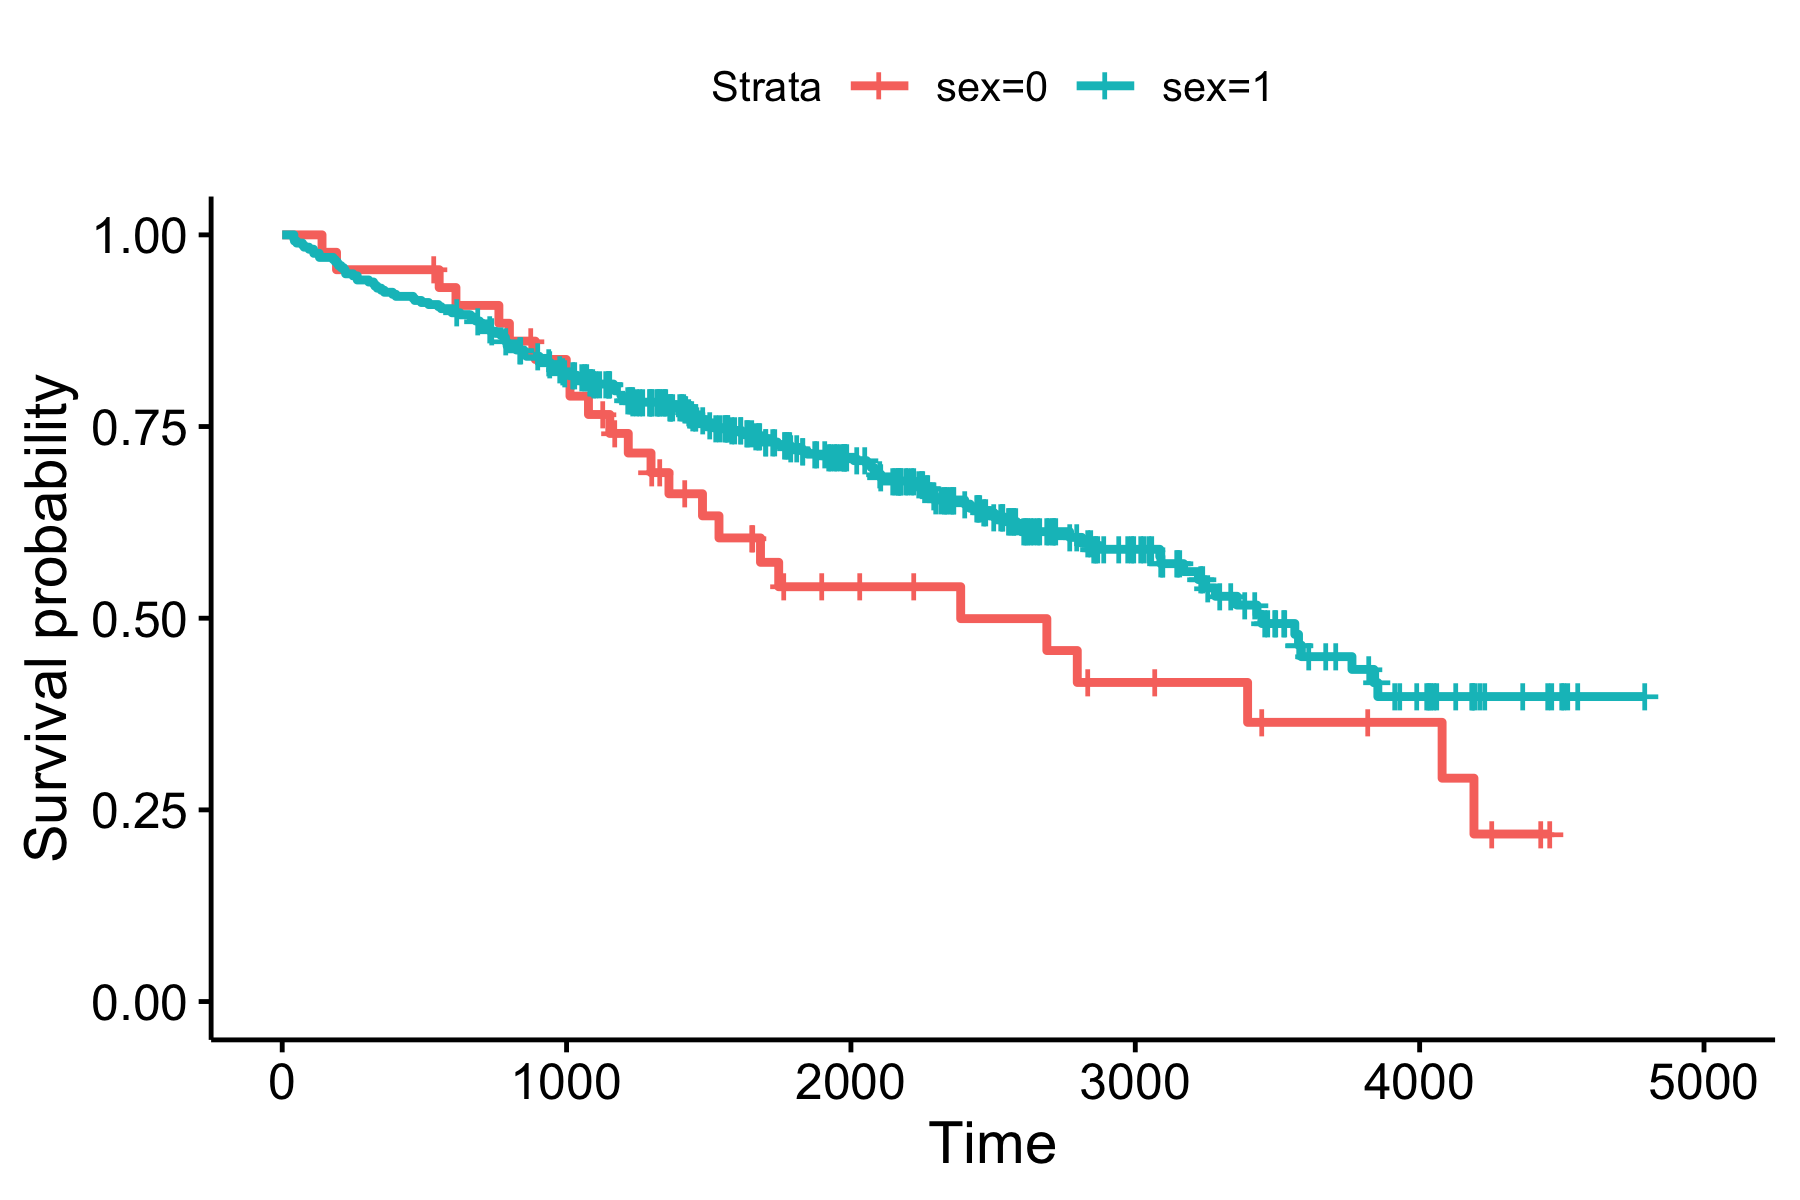
\includegraphics[width=0.48\textwidth]{img/rf-surv-example-1.png}
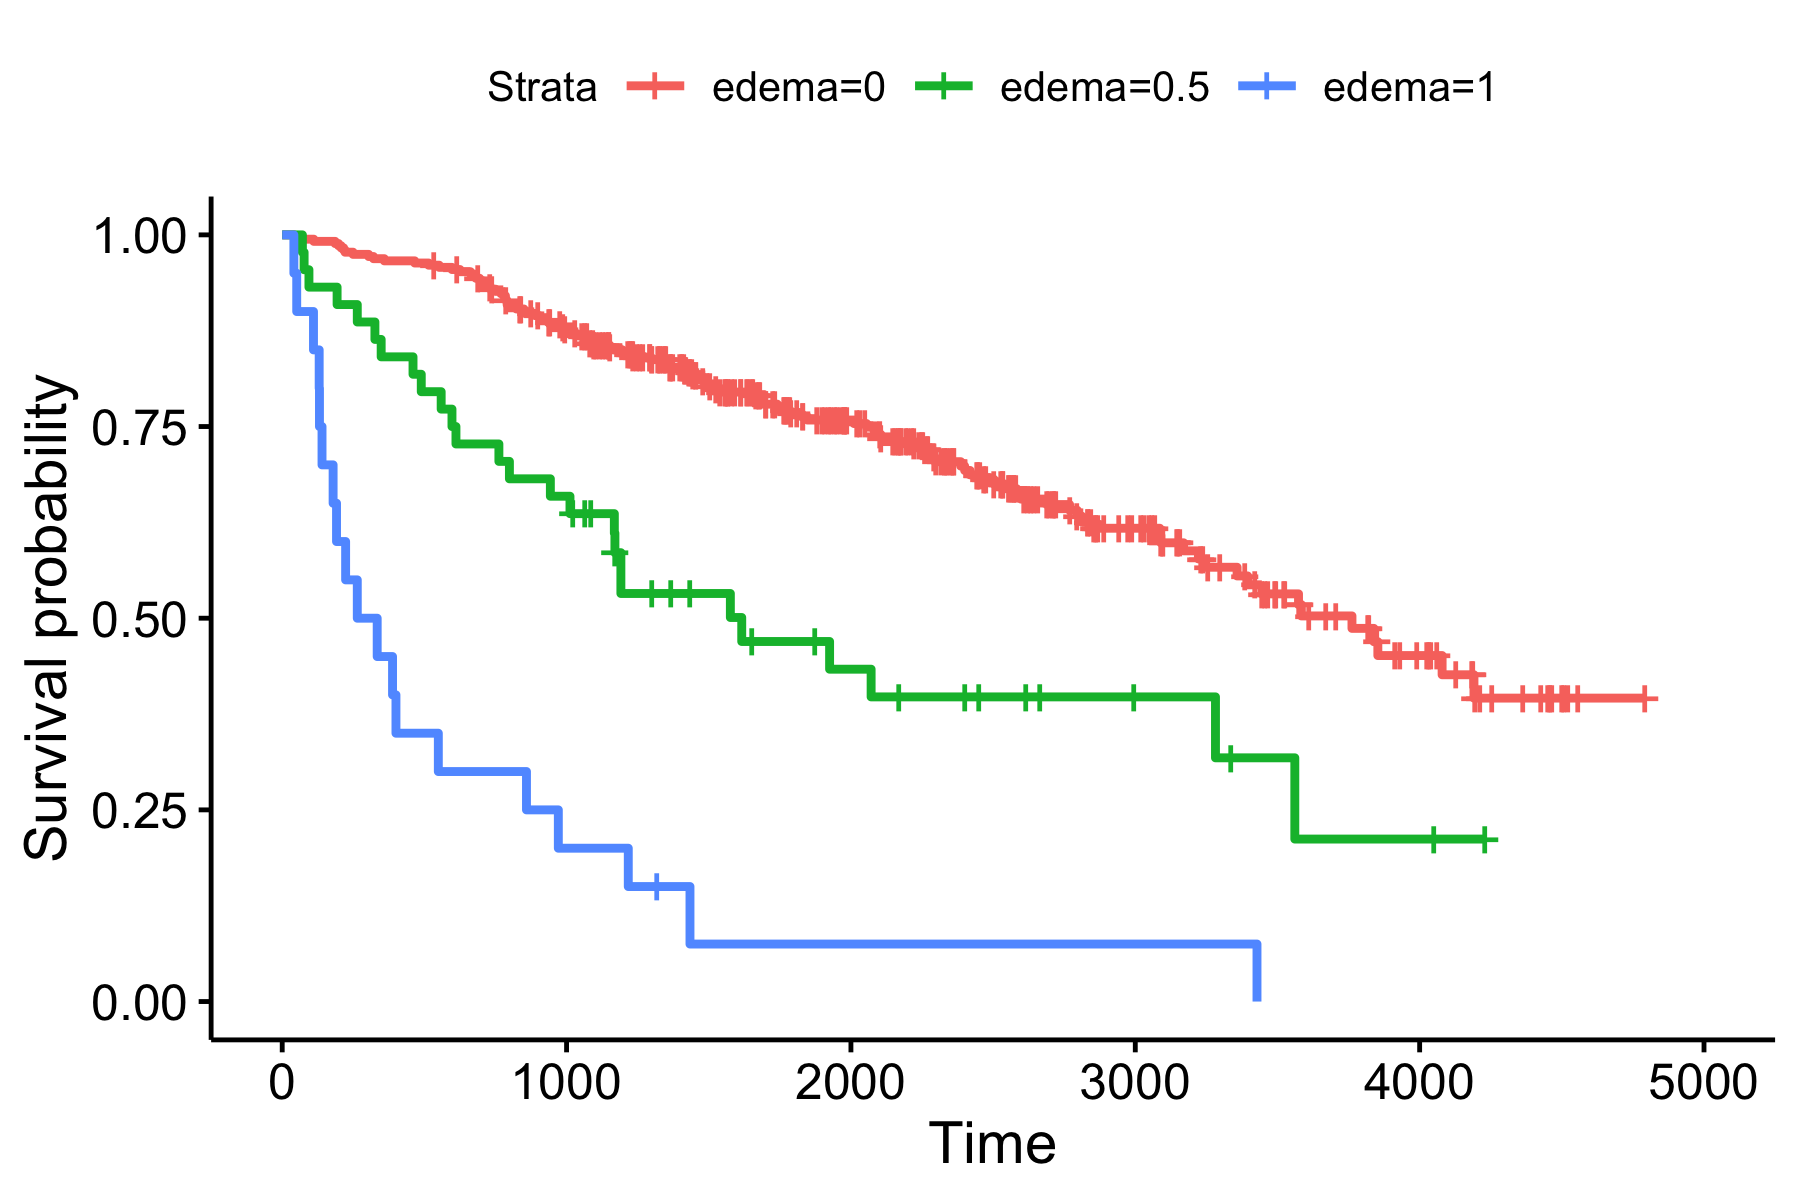
\includegraphics[width=0.48\textwidth]{img/rf-surv-example-2.png}
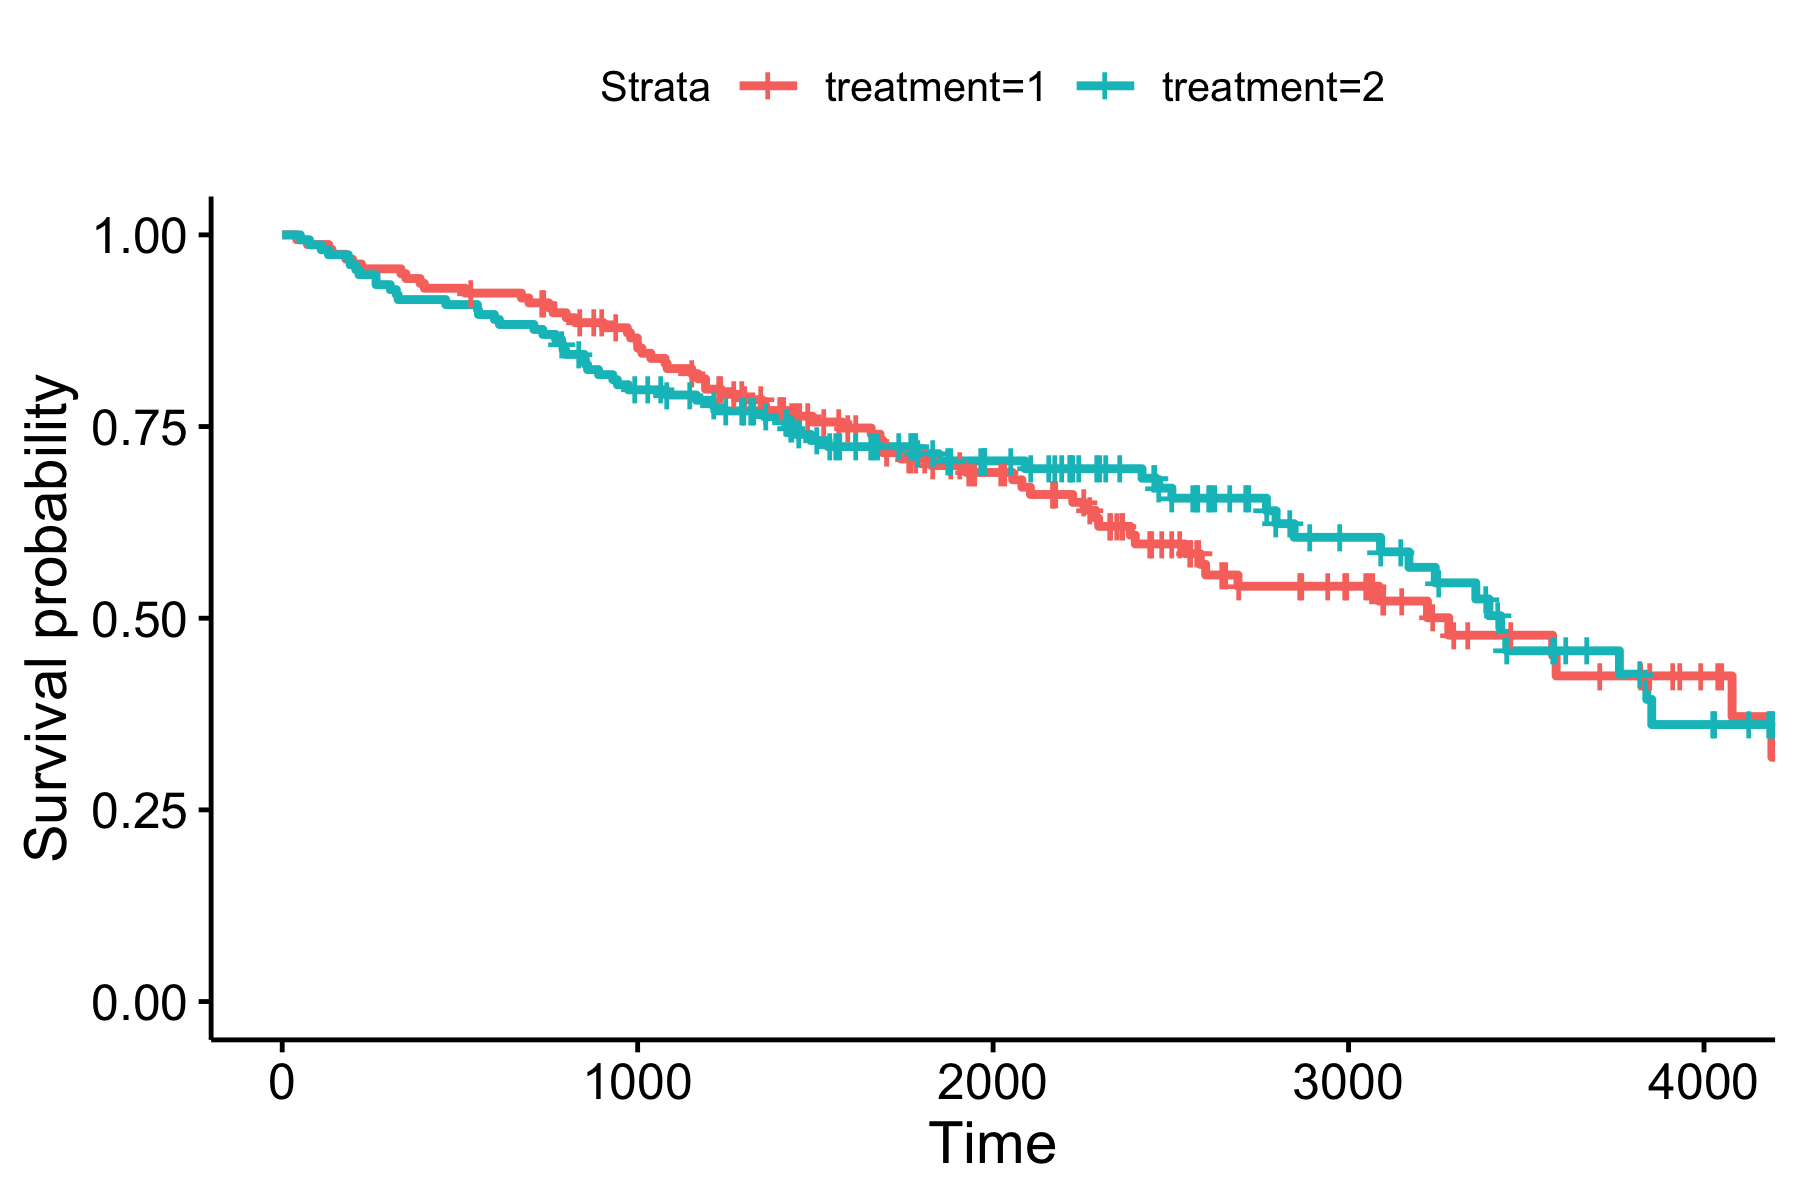
\includegraphics[width=0.48\textwidth]{img/rf-surv-example-3.png}
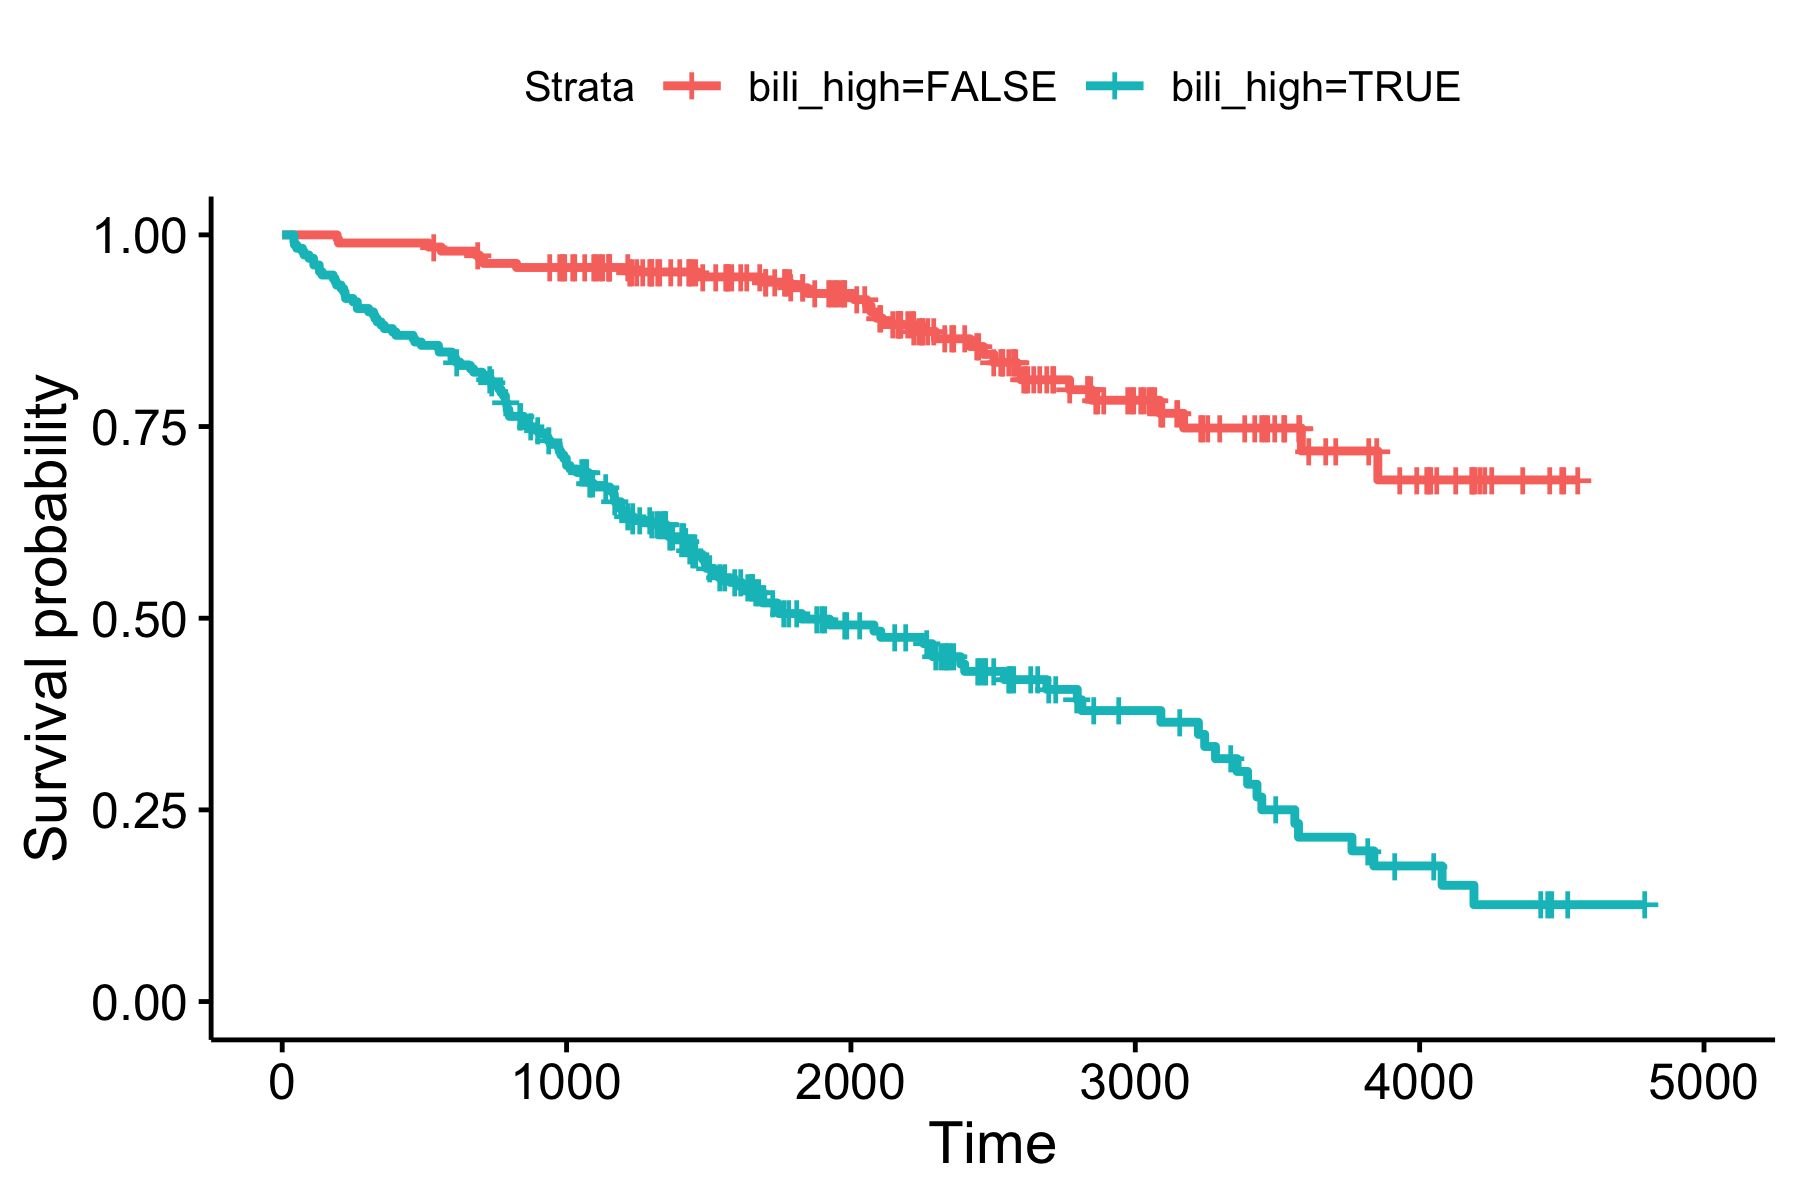
\includegraphics[width=0.48\textwidth]{img/rf-surv-example-4.png}
\end{center}

Say you wanted to build a decision tree to predict survival in PBC. You would want to choose splits for which survival looks very \emph{different} on either side of the split. This is analogous to choosing splits that increase the purity of the outcome (for classification) or reduce the variance of the outcome (regression). Speculate on how you might build such a tree. We will discuss the process of constructing \textbf{random survival forests} in much greater detail after we've seen a bit more survival analysis. 
\end{question}

\subsection{Creating Split Points}

Each node within a tree signifies a division of one of the predictors into two groups. \textbf{Deterministic splitting} means considering all possible splits and identifying the best one. For a numeric predictor, this involves considering all of the values of the predictor represented in the dataset; there may be as many as $n$ possible values, where $n$ is the number of training samples included in the tree. For a categorical predictor, this involves dividing the possible categories into two \textbf{complementary groups}. For example, the insurance cost dataset in Section~\ref{sect:reginsurance} contains a predictor \texttt{region} with four categories: northeast, southeast, southwest, and northwest. Each split decision must consider all $2^{k-1}-1$ possible divisions\footnote{This comes from taking $2^k$ (total combinations of $k$ categories), subtracting $2$ (all in or all out, neither of which is possible), and then dividing the whole thing by $2$ (because the ordering of the groups doesn't matter). $(2^k - 2)/2 = 2^{k-1}-1$} of those categories, where $k$ is the number of categories. For \texttt{region}, the possible splits are:

\begin{center}
{\small \tt
\begin{tabular}{ll}
Group 1 & Group 2 \\
\midrule
NE, SE, SW & NW \\
NE, SW, NW & SE \\
NE, SE, NW & SW \\
SE, SW, NW & NE \\
NE, SE & NW, SW \\
NE, SW & NW, SE \\
NE, NW & SE, SW \\
\end{tabular}
}
\end{center}

\vspace{3mm}

Deterministic splitting becomes problematic when the number of possible splits is large. In that case, software packages often employ \textbf{random splitting}, in which a predetermined number of possible splits (the exact number is set using a parameter) are randomly chosen from among all the possibilities. 

\vspace{5mm}

\begin{question}{}
A known issue with decision trees is their tendency to prefer to split on continuous predictors over discrete predictors. Why do you think this is? It can be avoided, in part, by using random splitting with a fixed number of possible splits. 
\end{question}

\subsection{Bag Size and Number of Predictors}

Each tree in a random forest is built using a ``bagged'' sample of $n$ training examples from the original $N$ examples. Typically around $2/3$ of training examples are used per tree, but most software packages include a parameter that allows the user to set this value. In addition, at each split, a tree considers only a randomly-chosen subset of $p$ predictor variables; the default number is usually $\sqrt{P}$ (for classification problems) or $P/3$ (for regression problems), where $P$ is the total number of predictors. In software, this will also be a settable parameter. Usually it's fine to leave these parameters at their default values.

\vspace{5mm}

\begin{question}{}
For an ensemble to be more accurate than any of its individual members, the learners comprising the ensemble must be \emph{accurate} and \emph{diverse}. Accuracy means that the learners must perform better than random on their designated task. Diversity means that the classifiers must make different errors on new data points. How do the parameters $n$ and $p$ impact diversity? How does the way the trees are trained ensure accuracy?
\end{question} 

\subsection{Node Size and Tree Depth}

Software packages generally allow the user to control the growth of individual trees within a random forest by specifying node size and tree depth parameters. The \textbf{node size} parameter governs the minimum number of training samples present at a node for a split to be considered. The \textbf{tree depth} parameter governs the maximum number of connections between the root of the tree and one of its leaves. A split at a particular node will only be considered when there is still some impurity in the outcome at that node (see Chapter~\ref{chapter:decisiontrees}) and when:
\begin{enumerate}
\item The current tree depth is less than the maximum allowed tree depth.
\item The number of samples at a node is at least 2x the minimum node size (since a binary split on a smaller node would result in leaves with less than the minimum required node size).
\end{enumerate}

%%%%%%%%%%%%%%%%%%%%%%%%%%%%%%%%%%%%%%%%%%%%%%%%%%%%%%%%%%%%%%%%%%%%%%%%%%%%%%%%%%

\section{The Out-of-Bag Error}

The random forest will report a number called the \textbf{out-of-bag (OOB) error} as it runs. To calculate OOB error, each tree makes a prediction for each of the training samples \emph{not} used in its construction. This provides an ongoing estimate of the generalization error of the forest.

Here is an OOB error plot for the random classification forest built on the Wisconsin Breast Cancer dataset:

\begin{center}
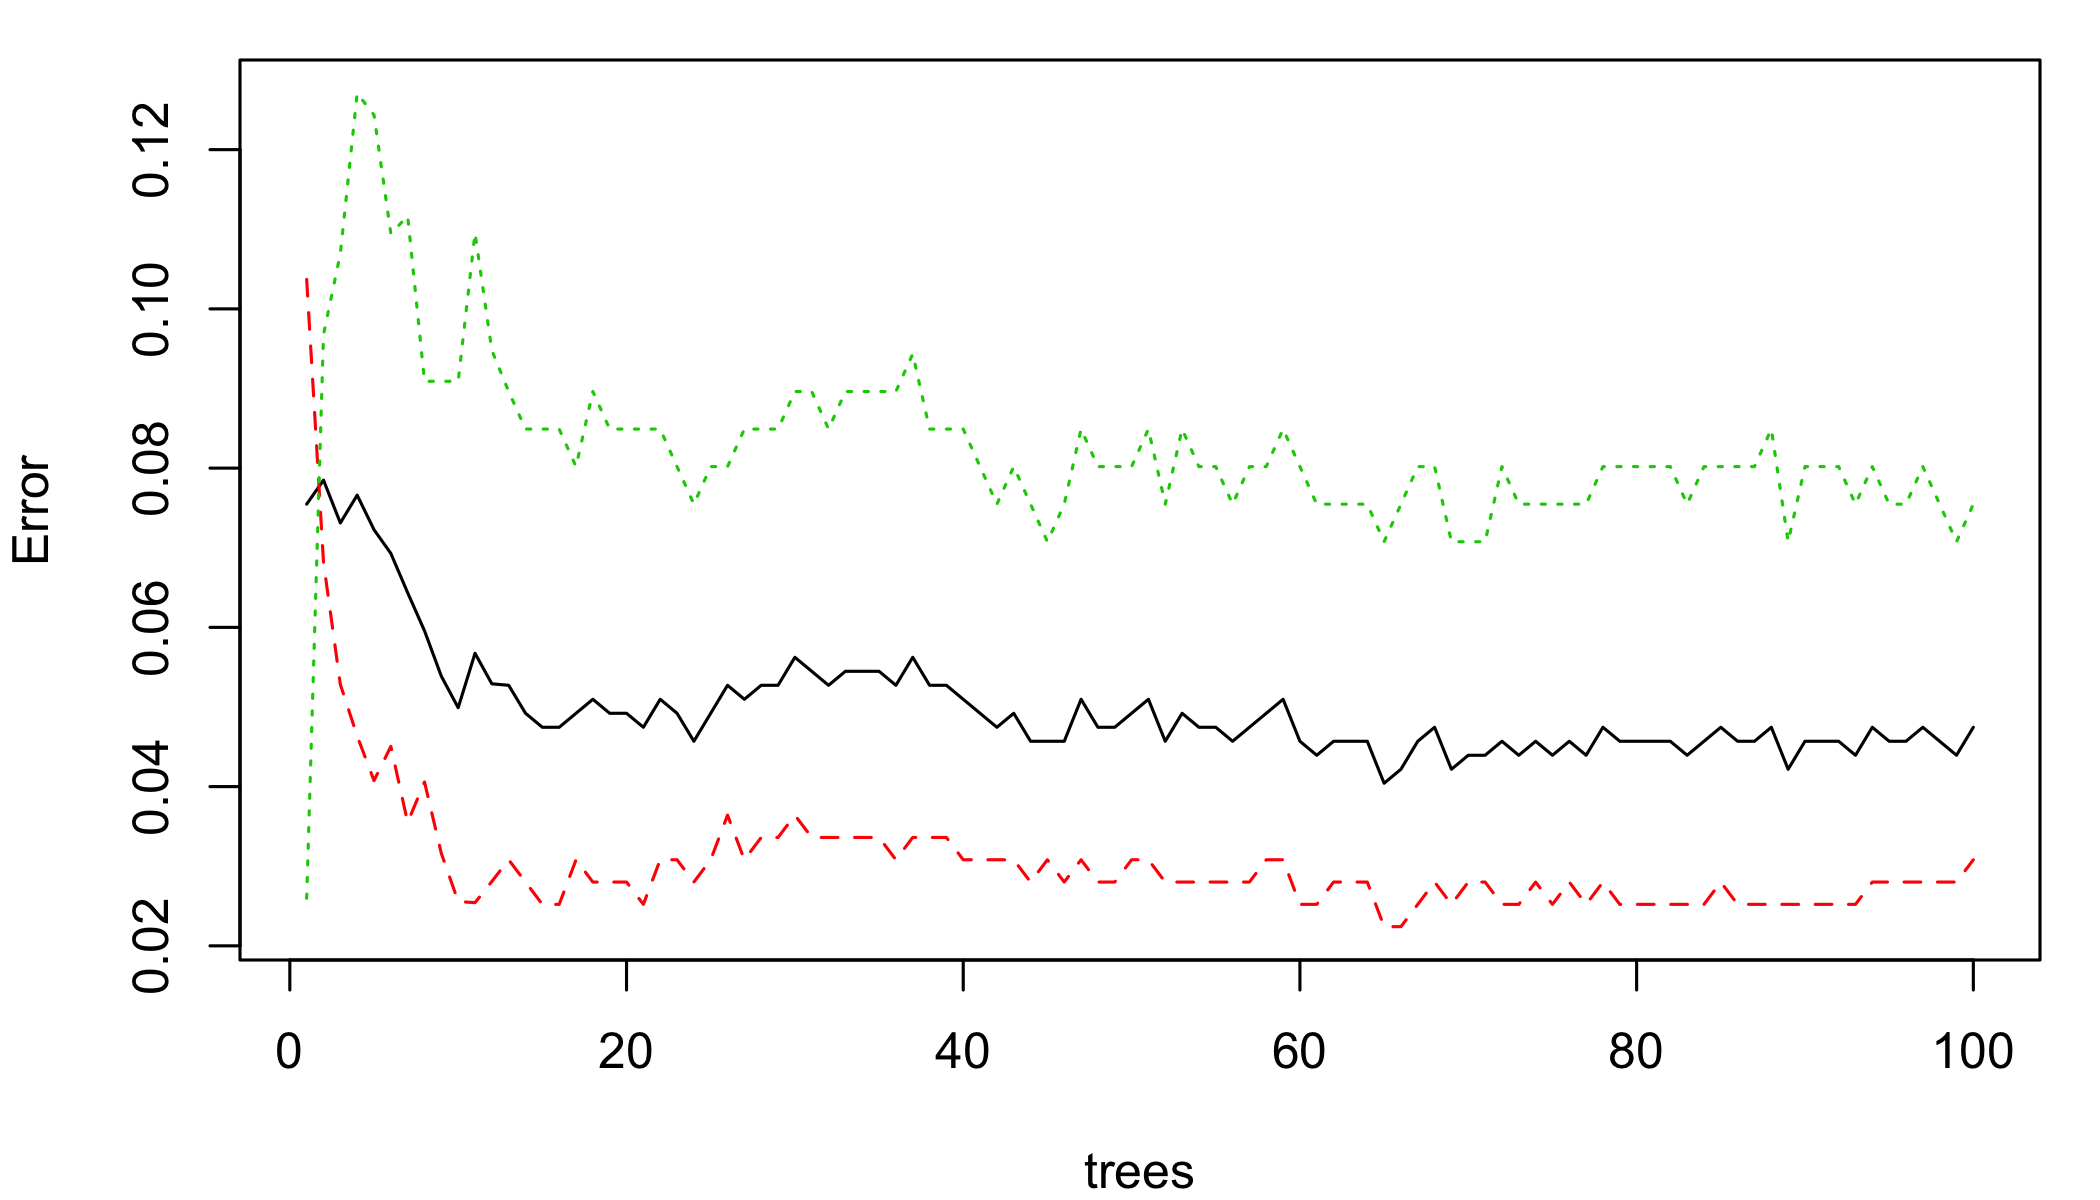
\includegraphics[width=0.7\textwidth]{img/oob-classification-wisc.png}
\end{center}
The black line shows the overall OOB error (the percent of OOB points misclassified) after the addition of each new tree. The red line shows the OOB error for points of class 1, which in this case is $B$ (benign), and the green line shows the OOB error for points of class 2, which in this case is $M$ (malignant).

\vspace{4mm}

\begin{question}{}
What does it mean that the green line is so much higher than the red line? What does this tell you about the relative rates of false positives and false negatives for this random forest?
\end{question}

\begin{question}{}
Here is the final \textbf{confusion matrix} for the Wisconsin Breast Cancer random forest. 
\vspace{-3mm}
\begin{center}
{\tt
\begin{tabular}{lrrr}
&    B  &  M  & class.error \\
B & 346 & 11 & 0.03081232 \\
M & 16 & 196 & 0.07547170 
\end{tabular}
}
\end{center}
\vspace{-3mm}
It is probably more important to avoid false negatives ($M$ tumors that are classified as $B$) than false positives. Speculate on ways in which you could force the forest to produce a lower rate of false negatives, even if it means increasing the number of false positives. 
\end{question}

For regression forests, the OOB error is calculated differently. It is defined as the mean square error among the OOB samples. The square root of this error is the average absolute value of the difference between the predicted and actual costs. 
\begin{center}
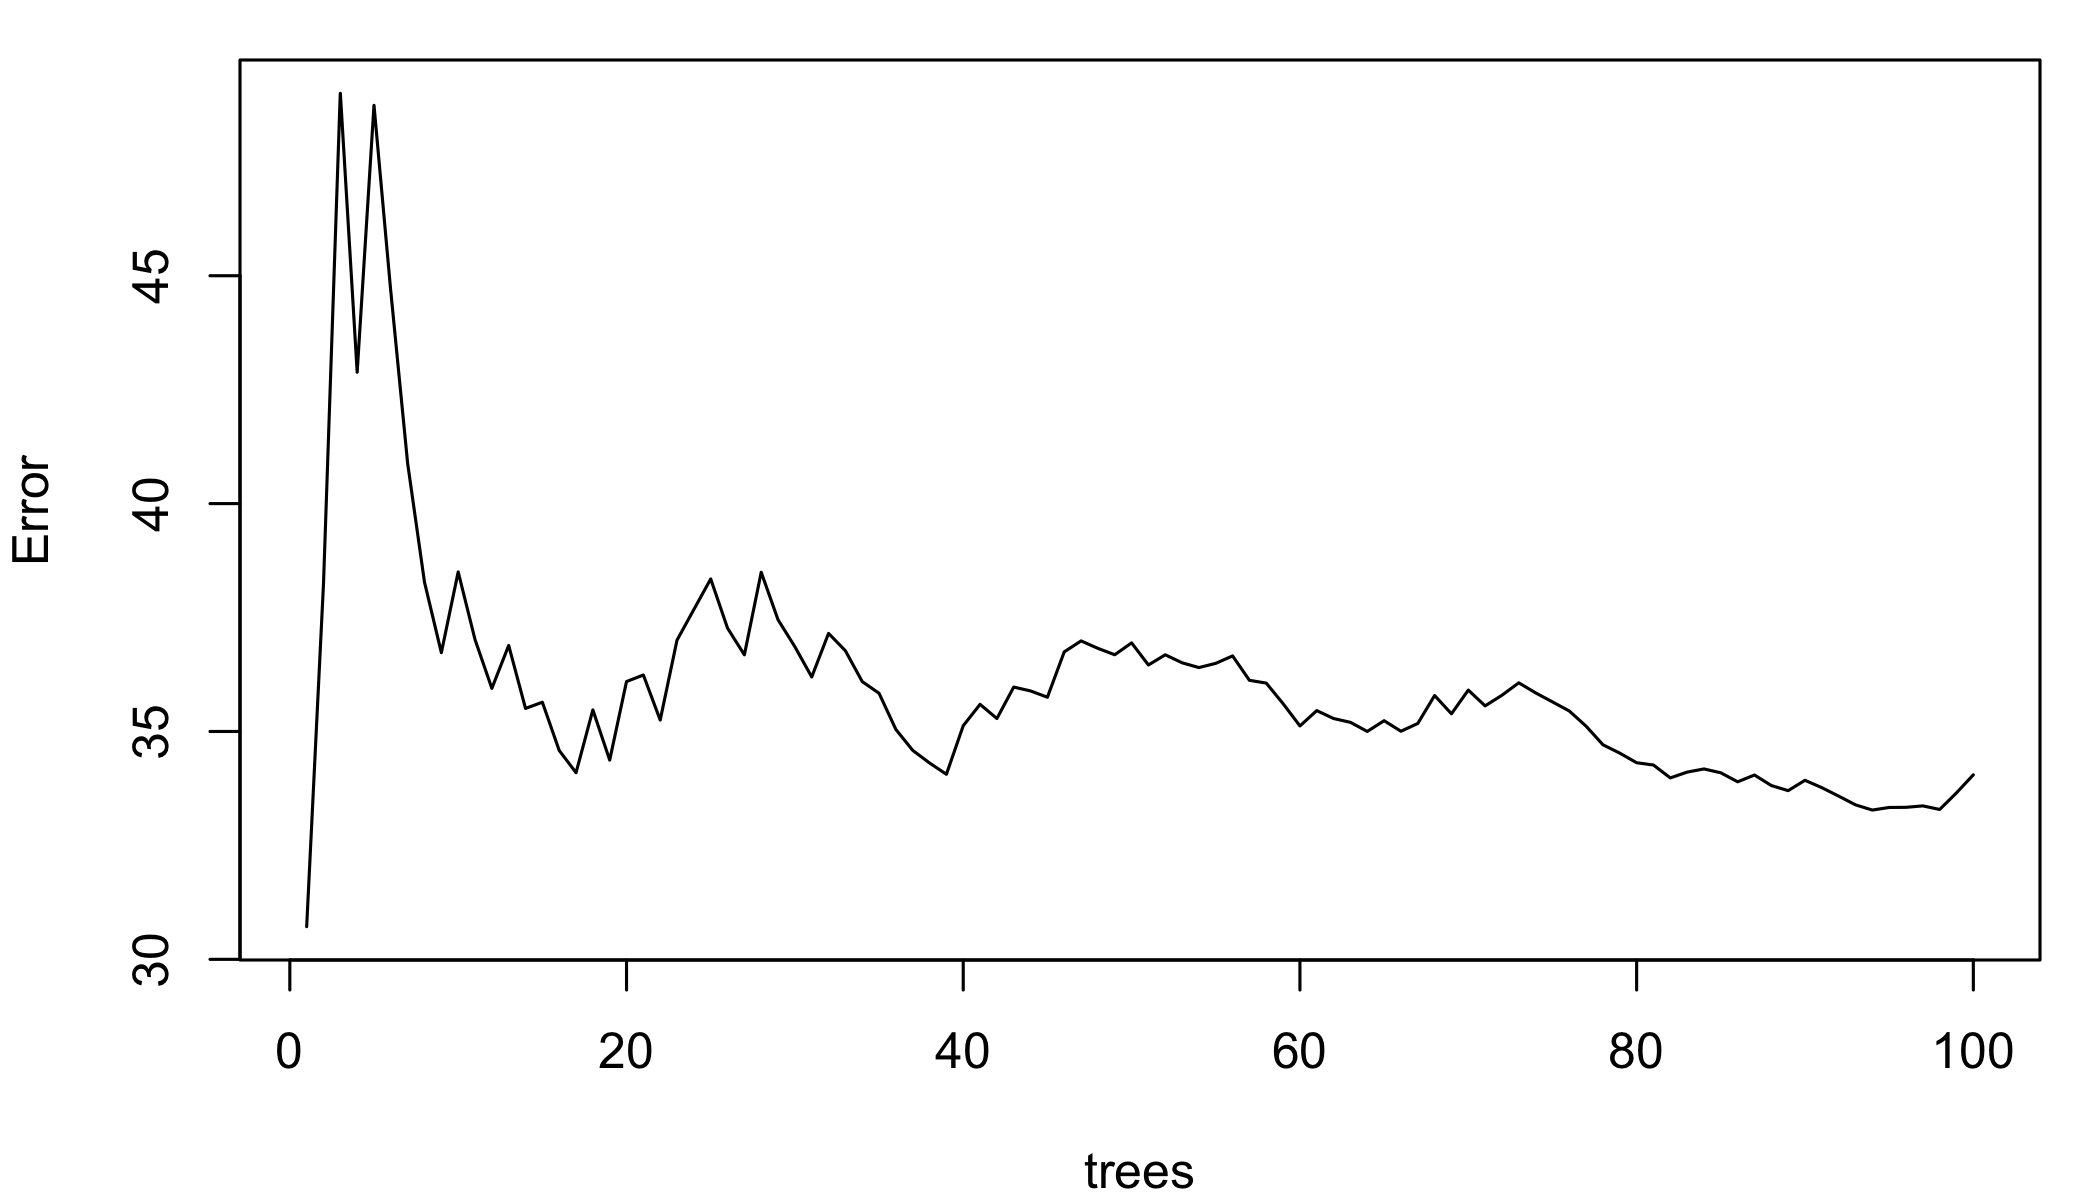
\includegraphics[width=0.7\textwidth]{img/oob-classification-insur.png}
\end{center}

%%%%%%%%%%%%%%%%%%%%%%%%%%%%%%%%%%%%%%%%%%%%%%%%%%%%%%%%%%%%%%%%%%%%%%%%%%%%%%%%%%

\section{Variable Importance Measures}

One of the main disadvantages of random forests is their lack of clarity around which variables are ``important''. In a regression model, the model output contains hypothesis tests and coefficients for each variable that provide the user with an interpretable importance ranking. Nothing this simple exists for random forests. However, there are some heuristics for ranking variables. These fall into two camps. 

\subsection{Impurity-Based Importance}

Trees are built by choosing splits that reduce uncertainty, or impurity, in the outcome. This impurity reduction is a measure of how much splitting on that variable ``helps'' in purifying the outcome. One way to measure the importance of a variable, therefore, is to average the decrease in node impurity across all splits involving that variable, across all trees in the random forest\footnote{Because splits occur at different heights, impurity reduction is typically weighted by how many samples reach a given node.}. This importance measure is called the \textbf{Mean Decrease in Impurity (MDI)}. It works no matter what your outcome is. Its main advantage is that because the reduction in impurity is what is already used to determine the splits, it requires very little additional computation.  

\subsection{Permutation-Based Importance}

An alternative way of measuring the importance of variable $j$ is to see how much it affects the predictive accuracy of trees across the whole forest. We assess this using the OOB samples. First the real OOB error is calculated (by running each sample through the trees for which it is OOB). Then the values of variable $j$ across the OOB samples are randomly permuted, and the OOB error is calculated again. We expect the OOB error to go up in the second case by an amount proportional to how important variable $j$ is. We then average this difference for each variable across all trees. This permutation-based importance measure is called the \textbf{Mean Decrease in Accuracy (MDA)}. Again, it works no matter what the outcome is. Its main advantage is that it is more interpretable than MDI. 

\vspace{4mm}

\begin{question}{}
Here is a variable importance plot for the Wisconsin Breast Cancer classification forest. Which side is MDI and which is MDA? Which variables are most and least important?
\begin{center}
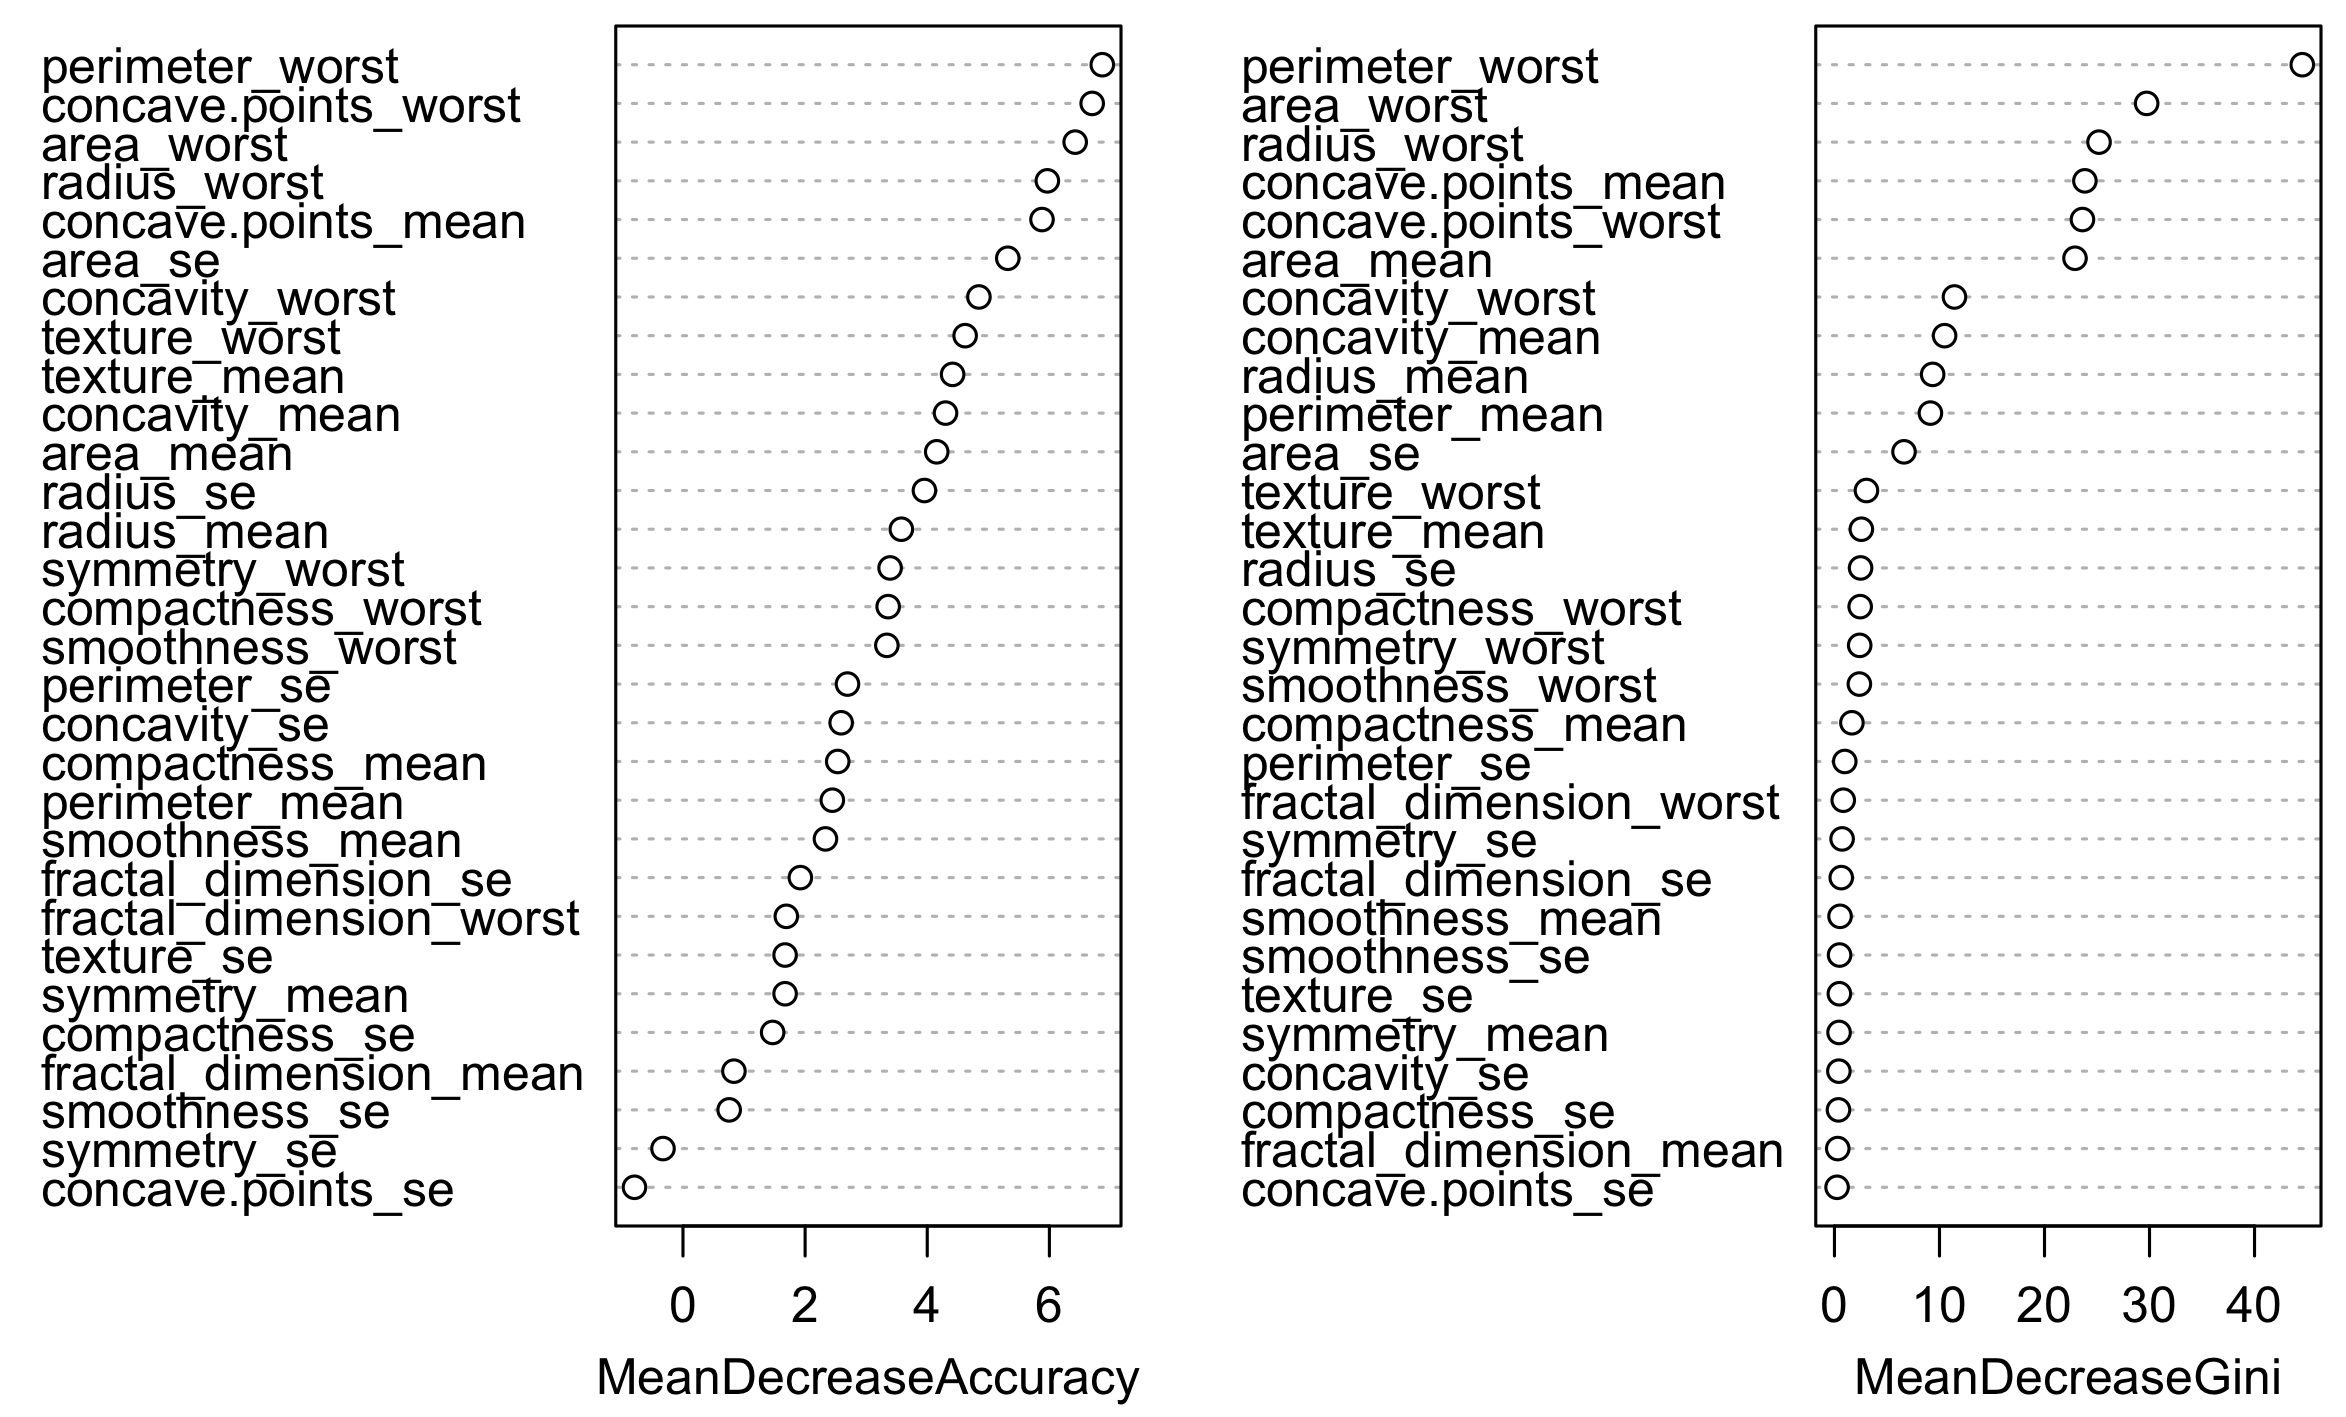
\includegraphics[width=0.85\textwidth]{img/vimp-classification-wisc.png}
\end{center}
\end{question}

\begin{question}{}
Here is a variable importance plot for the insurance cost dataset regression forest. Which side is MDI and which is MDA? Which variables are most and least important?
\begin{center}
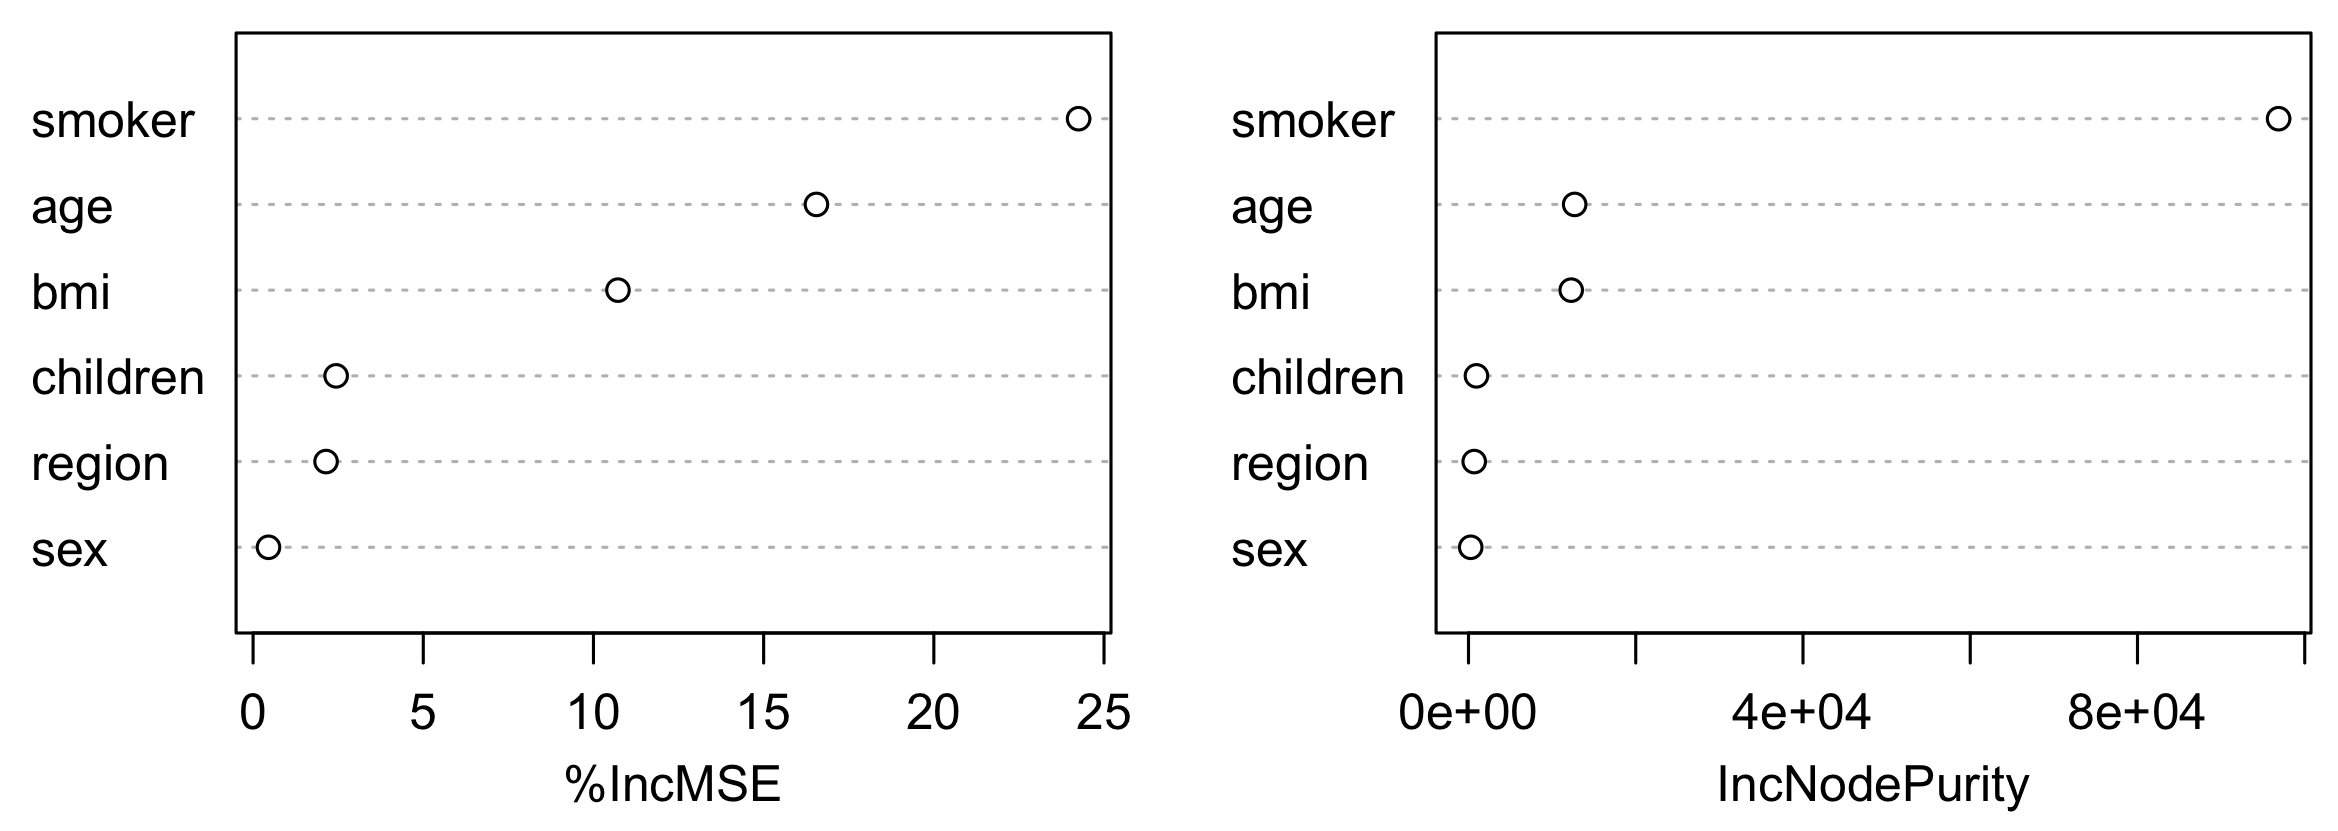
\includegraphics[width=0.85\textwidth]{img/vimp-classification-insur.png}
\end{center}
\end{question}

%%%%%%%%%%%%%%%%%%%%%%%%%%%%%%%%%%%%%%%%%%%%%%%%%%%%%%%%%%%%%%%%%%%%%%%%%%%%%%%%%%

\section{A Note on Software Packages}

As we have seen in Chapter~\ref{chapter:decisiontrees}, there are many different ways to build and optimize decision trees. There are even more ways to build and optimize random forests. This chapter uses the \texttt{randomForest} R package by Andy Liaw, a faithful implementation of the original random forest implementation suggested by Breiman (2003), as well as \texttt{randomForestSRC}, a faster and more recent package by Ishwaran and Kogalur that provides a unified interface for random forest-based classification, regression, and survival analysis. The \texttt{scikit-learn} package in Python provides implementations of random forests for both classification and regression. 
